In contesti a basso impatto antropico, nei fiumi a morfologia intrecciata dove il livello di disturbo indotto dalle piene non è eccessivo è possibile trovare isole nell'alveo;
queste si formano e accrescono nel periodo compreso tra eventi di piena di una certa entità, mentre vengono erose dagli eventi idrologici sufficientemente intensi \squarecite{Gurnell:2001-island-formation}.
La presenza delle isole ha un importante ruolo ecologico: la varietà spaziale e temporale di ambienti presenti (pozze d'acqua, sorgenti e canali separati da aridi sedimenti, zone con vegetazione bassa e rada alternate con isole fitte e mature che si modificano tra e in seguito alle piene) crea un mosaico in continuo cambiamento che sostiene una forte biodiversità.
Inoltre, durante piene di piccola entità le piante influenzano l'accrescimento delle forme fluviali attraverso la ritenzione di sedimenti e materiale legnoso sia morto che vivo, inducendo così la successiva colonizzazione da parte di altre piante e la rimodellazione dei canali.

La presente tesi mira a studiare come cambiano le isole nel fiume Tagliamento in risposta al regime idrologico (successione di magre, piene \emph{bankfull}, \emph{flow pulses}).
L'obiettivo principale è la ricerca di una relazione tra le piene e la quantità di vegetazione erosa in seguito ad eventi idrologici sufficientemente intensi.
%, o che leghi i livelli con la quantità di legname che si ritrova in alveo dopo eventi di piena.
In via previsionale si cerca di rispondere all'esigenza di stimare in anticipo gli effetti che una piena può avere sulle isole.
\\
Inoltre si trovano traiettorie evolutive per quanto riguarda la larghezza e la percentuale di isole rispetto all'alveo attivo; si confrontano i dati ottenuti per un tratto di qualche chilometro con alcuni risultati da letteratura; si ottengono relazioni tra la forza della corrente (\emph{stream power}) e la quantità massima di isole presenti.
%Inoltre si trovano valori soglia del livello del pelo libero per l'erosione della vegetazione.
\\
Nel periodo di studio 2000-2018 si analizzano contemporaneamente immagini satellitari, ortofoto e rilievi aerei LiDAR al fine di distinguere la parte dell'alveo ricoperta da vegetazione; si considerano i dati di livello del pelo libero dell'acqua registrati da un idrometro per osservare le piene.
% e gli elementi legnosi (tronchi e accumuli di legno, \vref{fig:esempio-accumulo-1}).

%\begin{figure}
%	\centering
%	\begin{subfigure}[b]{0.52\textwidth}
%		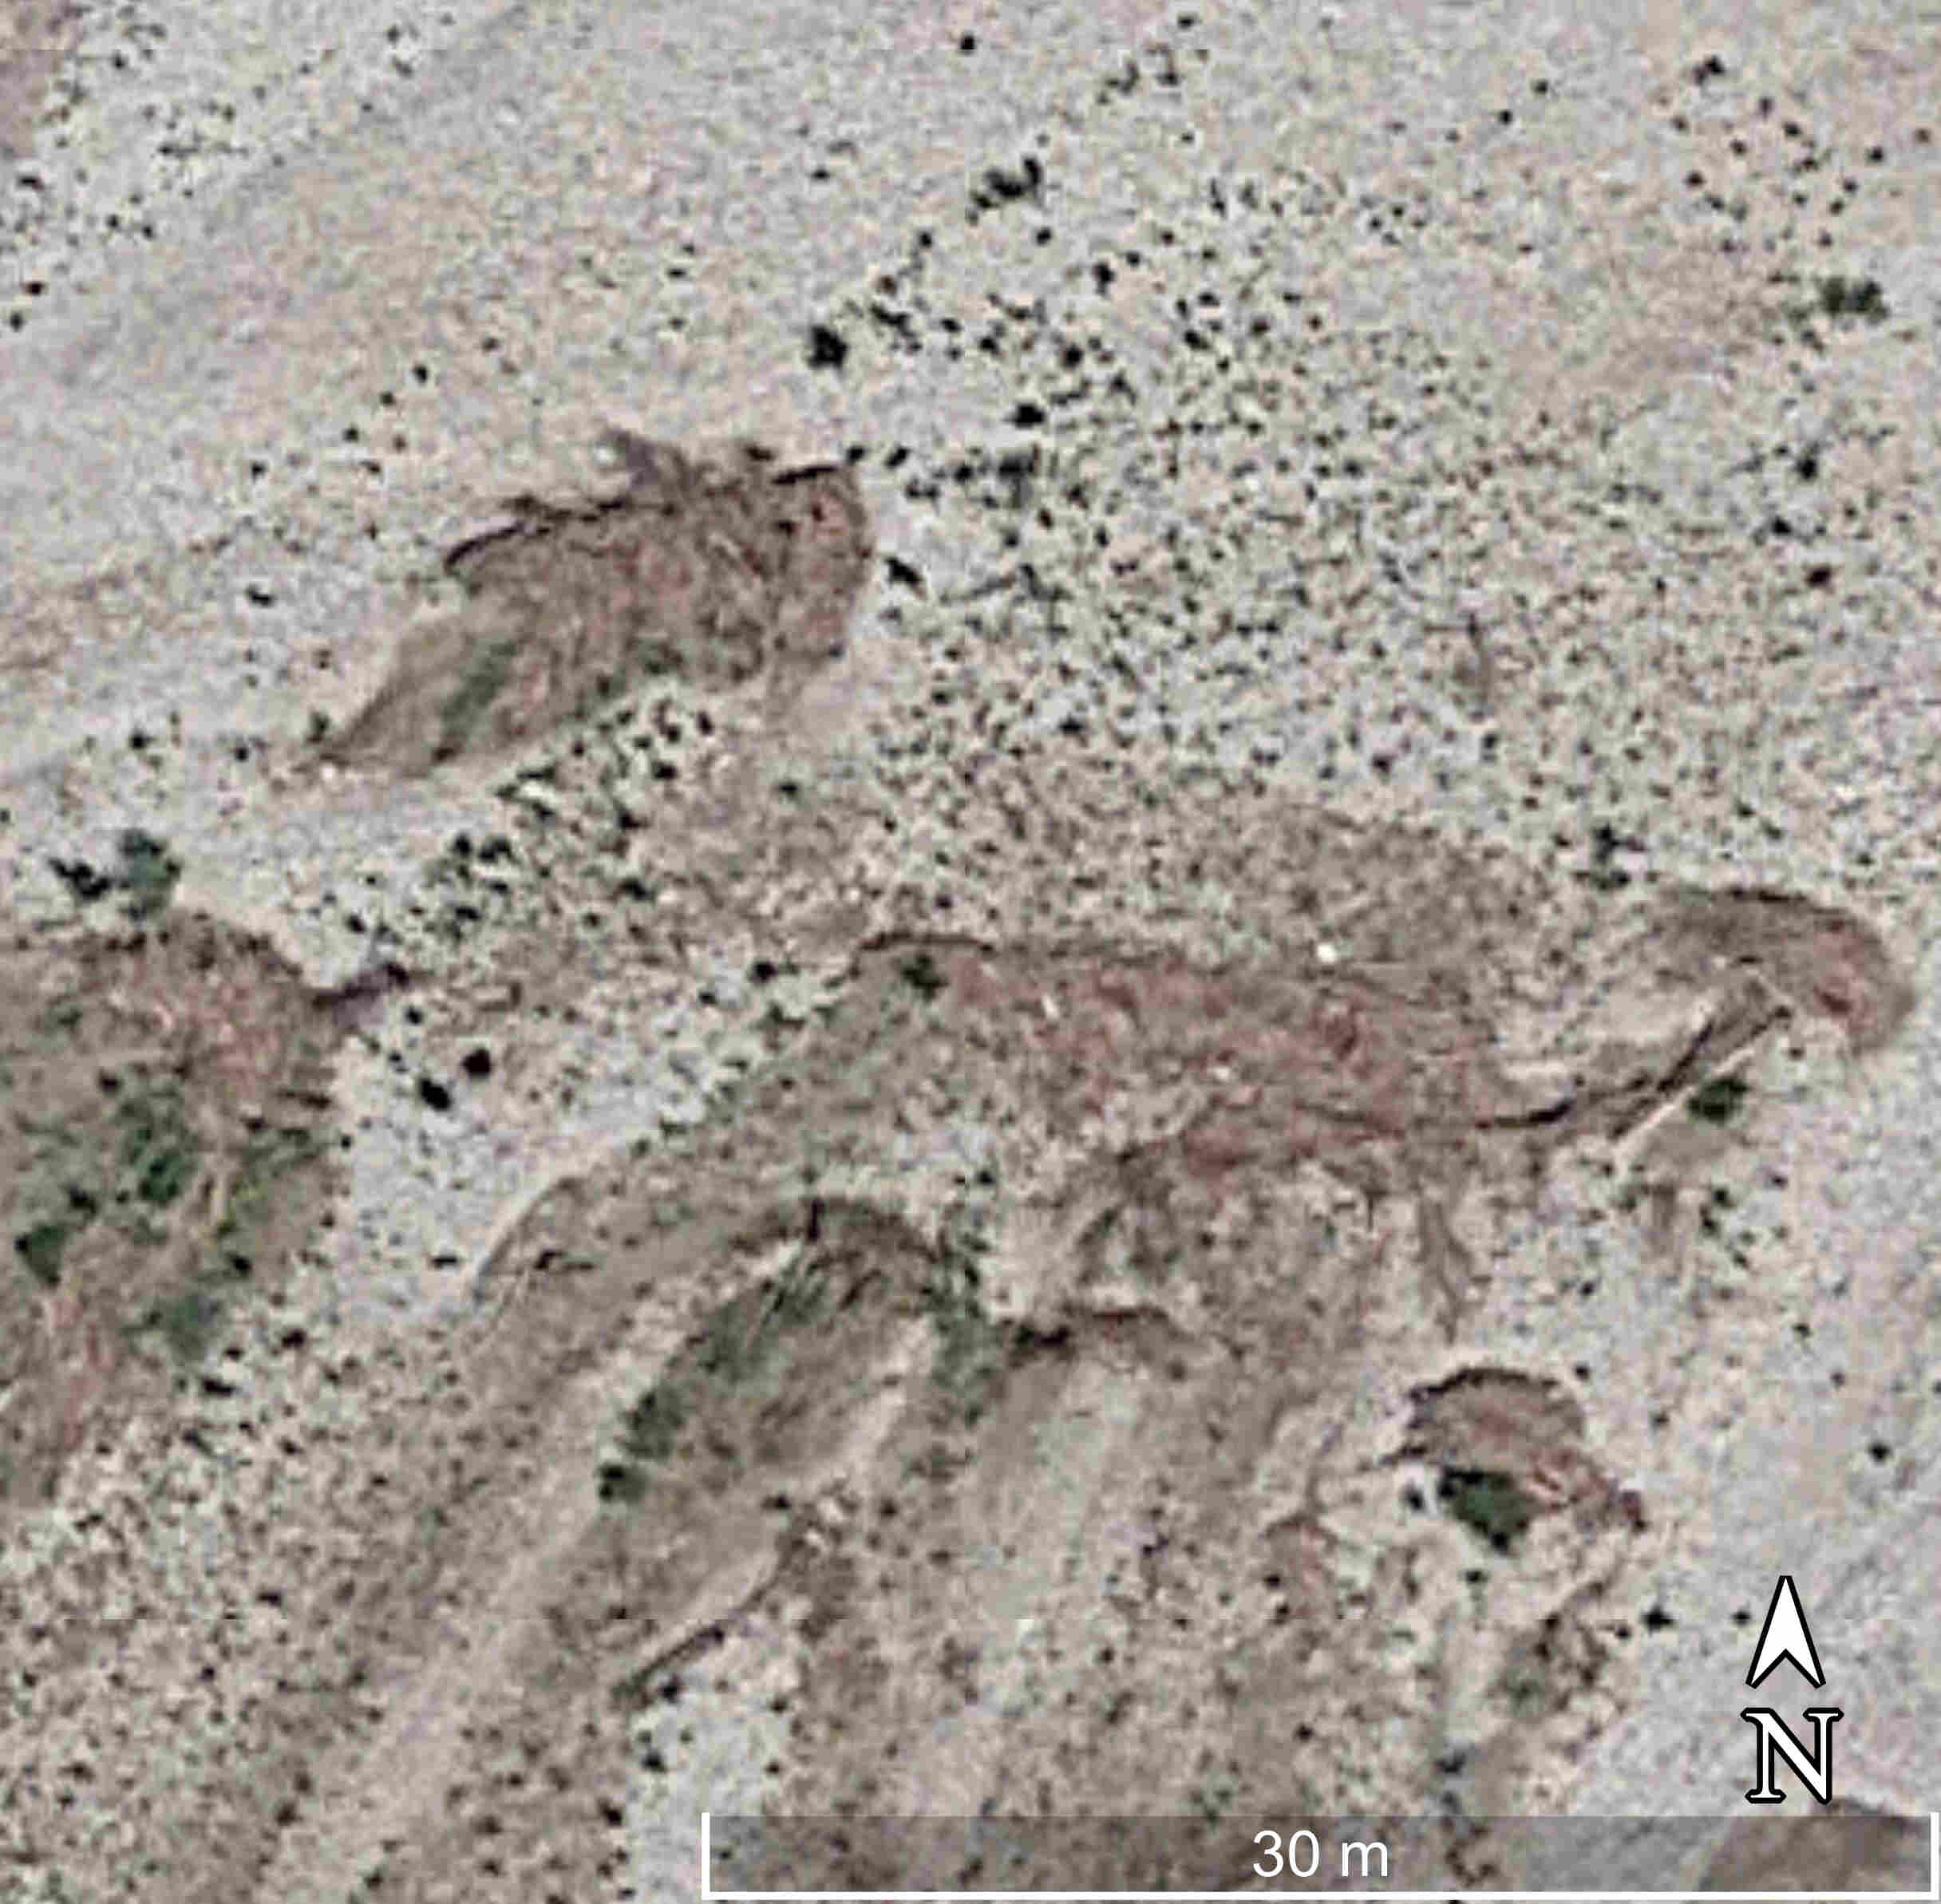
\includegraphics[width=\textwidth]{files/esempio_accumulo_sat_1.jpg}
%		\caption{immagine da Google Earth di accumuli di legno e tronchi in alveo (in marrone chiaro).}
%		\label{fig:esempio-accumulo-sat-1}
%	\end{subfigure}
%	\quad
%	\begin{subfigure}[b]{0.44\textwidth}
%		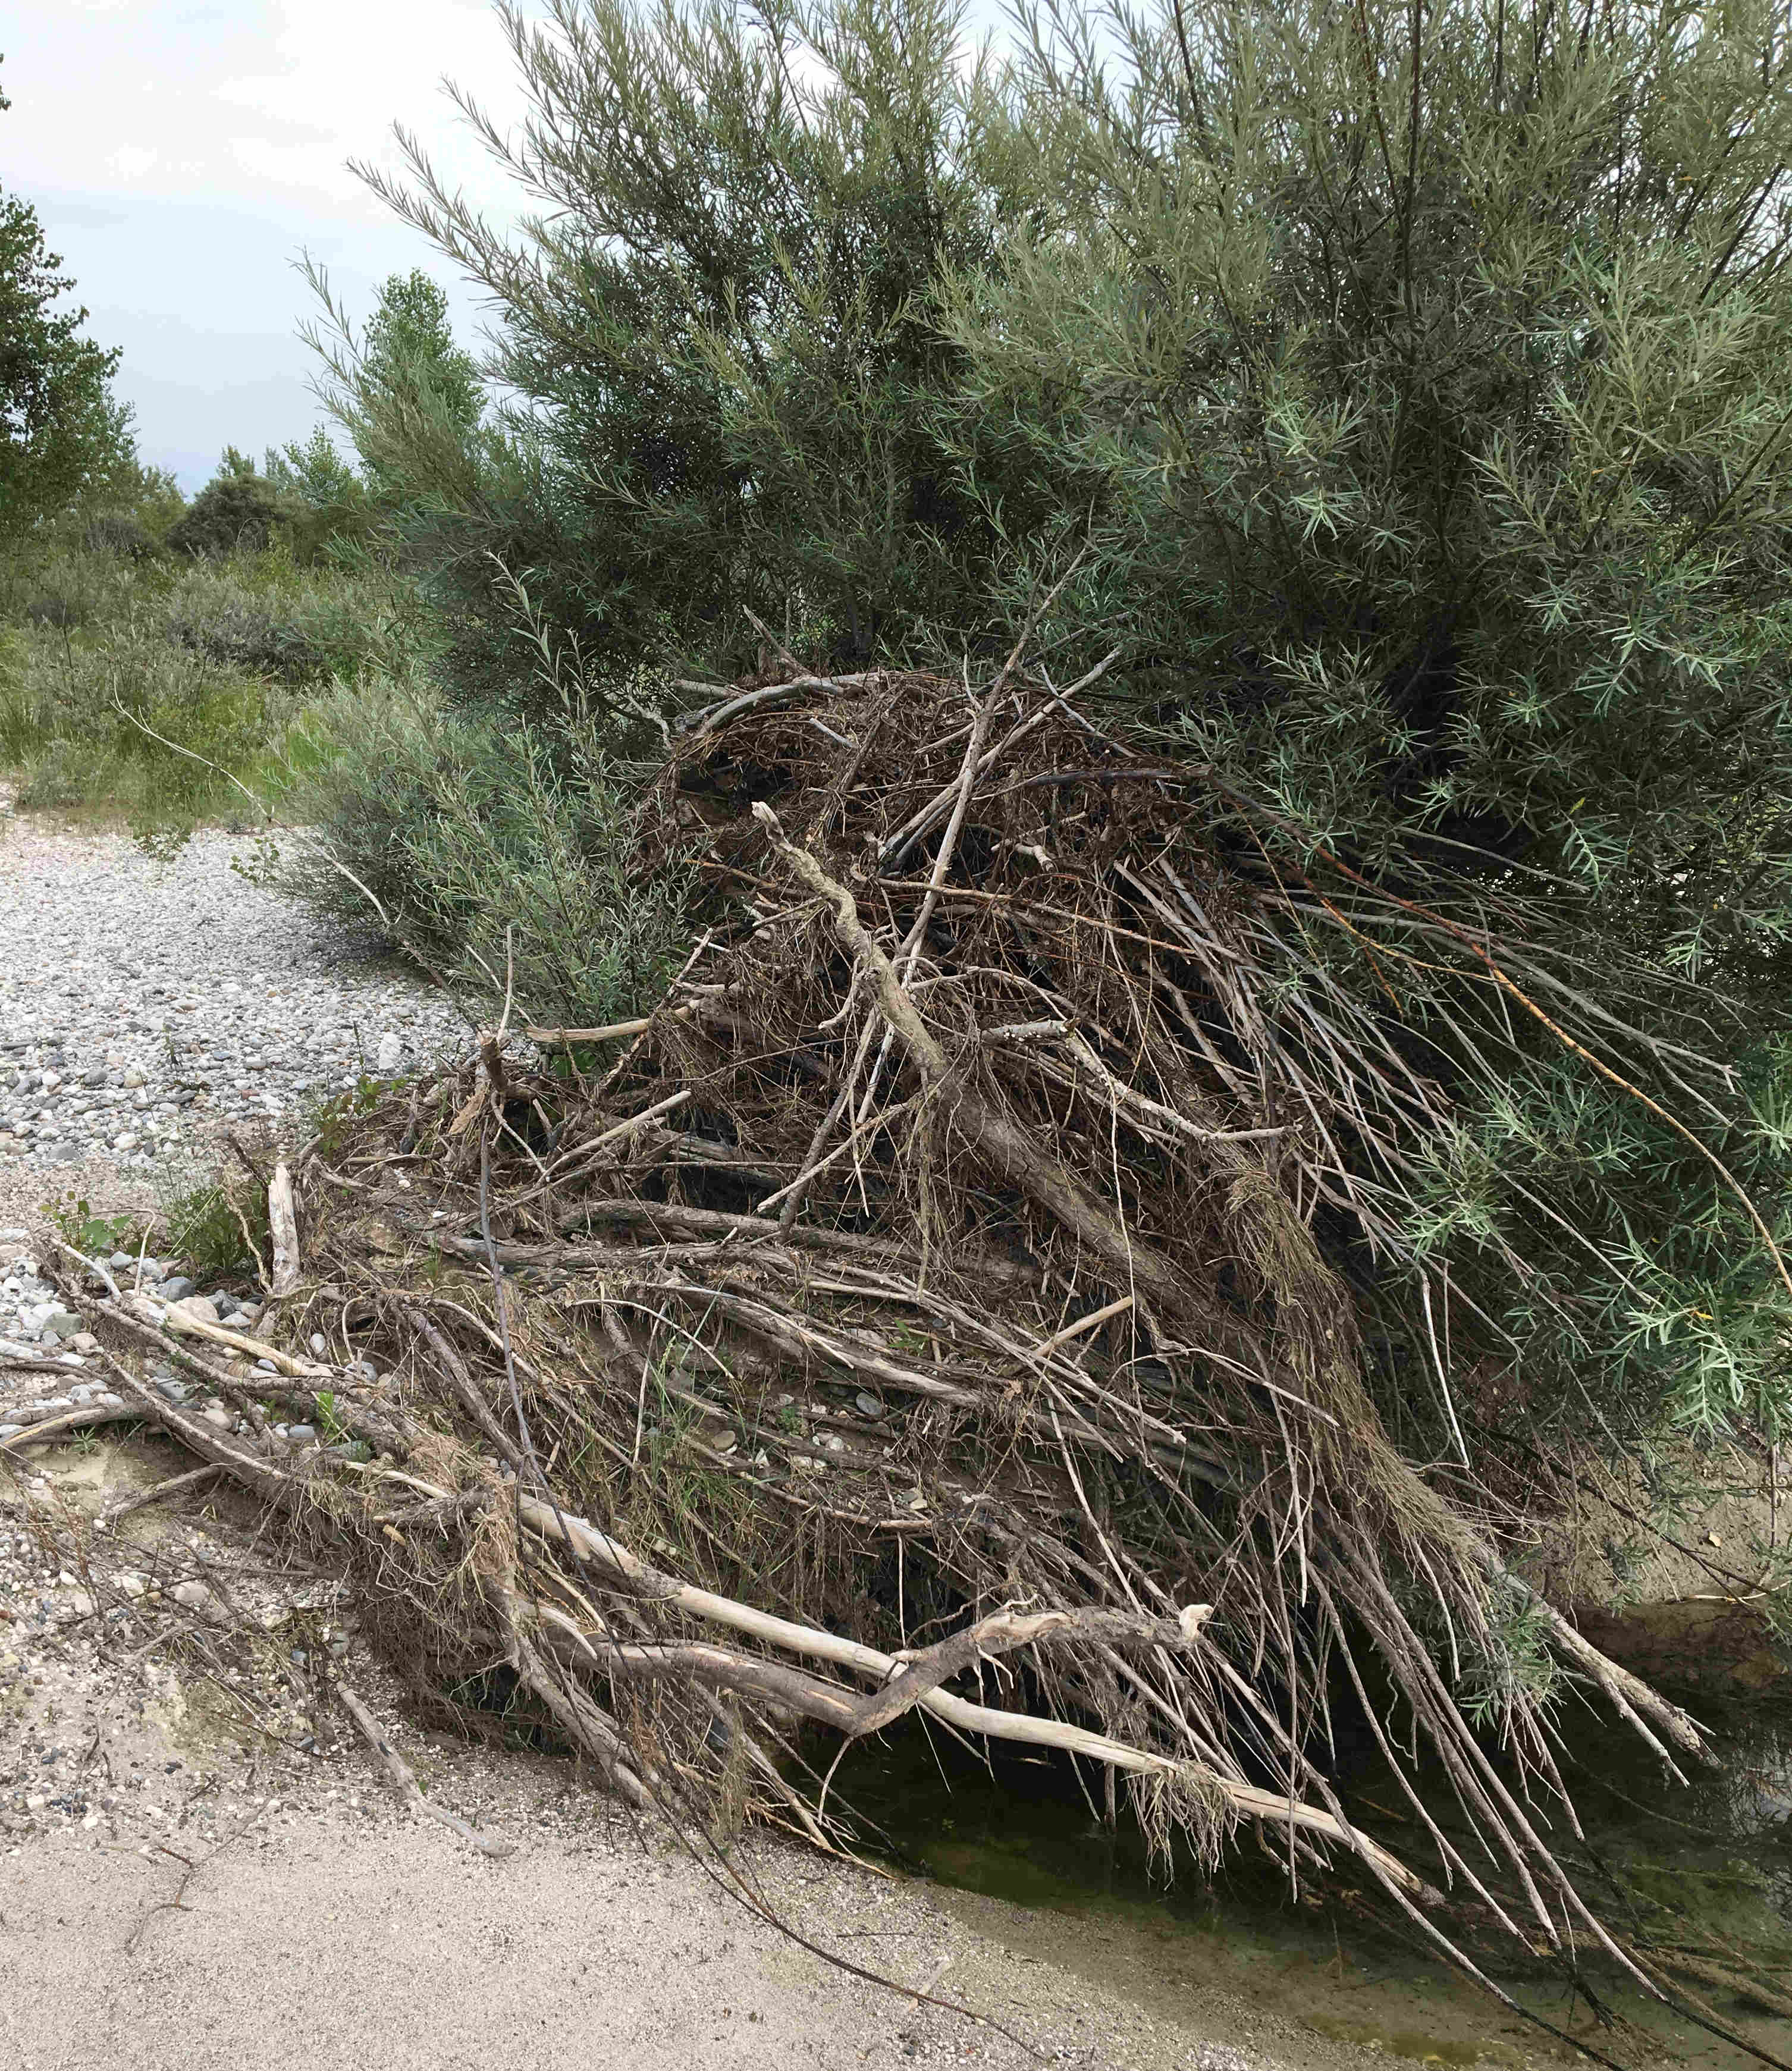
\includegraphics[width=\textwidth]{files/esempio_accumulo_1.jpg}
%		\caption{foto di un accumulo di tronchi sopra una pianta di salice.
%		Foto dell'autore.}
%		\label{fig:esempio-accumulo-1}
%	\end{subfigure}
%	\caption[immagine e foto di accumuli legnosi]{immagine e foto di accumuli legnosi. Il luogo della foto non corrisponde a quello dell'immagine.}
%\end{figure}


\section{Inquadramento dell'area di studio}
Il Fiume Tagliamento, situato nel Nord-Est italiano, è uno dei pochi fiumi alpini allo stato quasi naturale. 
Gli interventi effettuati sono arginature, derivazioni, pennelli, estrazione di ghiaia sia in tratti posti a monte che altri posti a valle; la loro entità è comunque tanto limitata da poter parlare di “contesto non gestito”.
Difatti il regime idrologico del Tagliamento presenta oscillazioni irregolari che hanno luogo ciclicamente ogni 6~mesi circa, probabilmente grazie alle precipitazioni autunnali e primaverili e allo scioglimento nivale \squarecite{Bertoldi:2009-2m}; inoltre le sponde sono colonizzate da vegetazione riparia lungo quasi tutto il suo corso, si accrescono e vengono erose. 
Questi due fatti indicano che le attività umane sul Tagliamento non sono tali da aver alterato o da alterare il regime del fiume.

Il bacino idrografico del Tagliamento, ampio circa~\SI{2900}{\kilo\m\tothe{2}}, si estende tra le province di Udine, Pordenone e Venezia.
Il suo corso di circa~\SI{170}{\kilo\m} presenta morfologia intrecciata (\emph{braided}, con canali multipli separati da barre e isole).
Nelle parti montane è confinato dai versanti; nella parte planiziale è libero, con tratti larghi diverse centinaia di metri, se non più di \SI{1}{\kilo\m};
A qualche decina di chilometri dalla foce il fiume si restringe assumendo prima una forma transizionale monocursale con larghezza sui \SIrange[range-phrase={-}]{300}{200}{\m} nei pressi di Madrisio~(UD);
infine meandriforme a Latisana~(UD) (larghezza intorno ai \SI{100}{\m}) fino alla foce, situata tra Bibione~(VE) e Lignano~(UD).
\\
Insieme alla variazione della morfologia del fiume si assiste ad un cambiamento nella granulometria: mentre la ghiaia predomina nella parte intrecciata ($d_{50} = \SI{4}{\centi\m}$ \squarecites{Bertoldi:2010-d50}{Sitzia:2016-d50}), a partire dal tratto meandriforme si trova solo sabbia sul fondo.
Questo mutamento di materiale trasportato riflette la riduzione della pendenza che si osserva dal tratto transizionale monocursale e che giustifica il passaggio da fiume “in ghiaia” a fiume “in sabbia”.
\\
Il regime delle precipitazioni consiste di circa \SI{2000}{\mm} all'anno in media con forti variazioni locali; i minimi di precipitazione si registrano durante l'inverno, mentre i massimi in primavera e in autunno. Si assiste anche ad eventi di breve durata e particolarmente intensi.
Il regime fluviale che ne risulta è di tipo \emph{flashy} pluvio-nivale con piene brevi ed intense così come piene di diversi giorni di durata.

Il tratto studiato è quello intrecciato multicanale compreso tra Tolmezzo~(UD) e Madrisio~(UD) (\vref{fig:overview,fig:overview-sat}). 
%
\begin{figure}
	\centering
	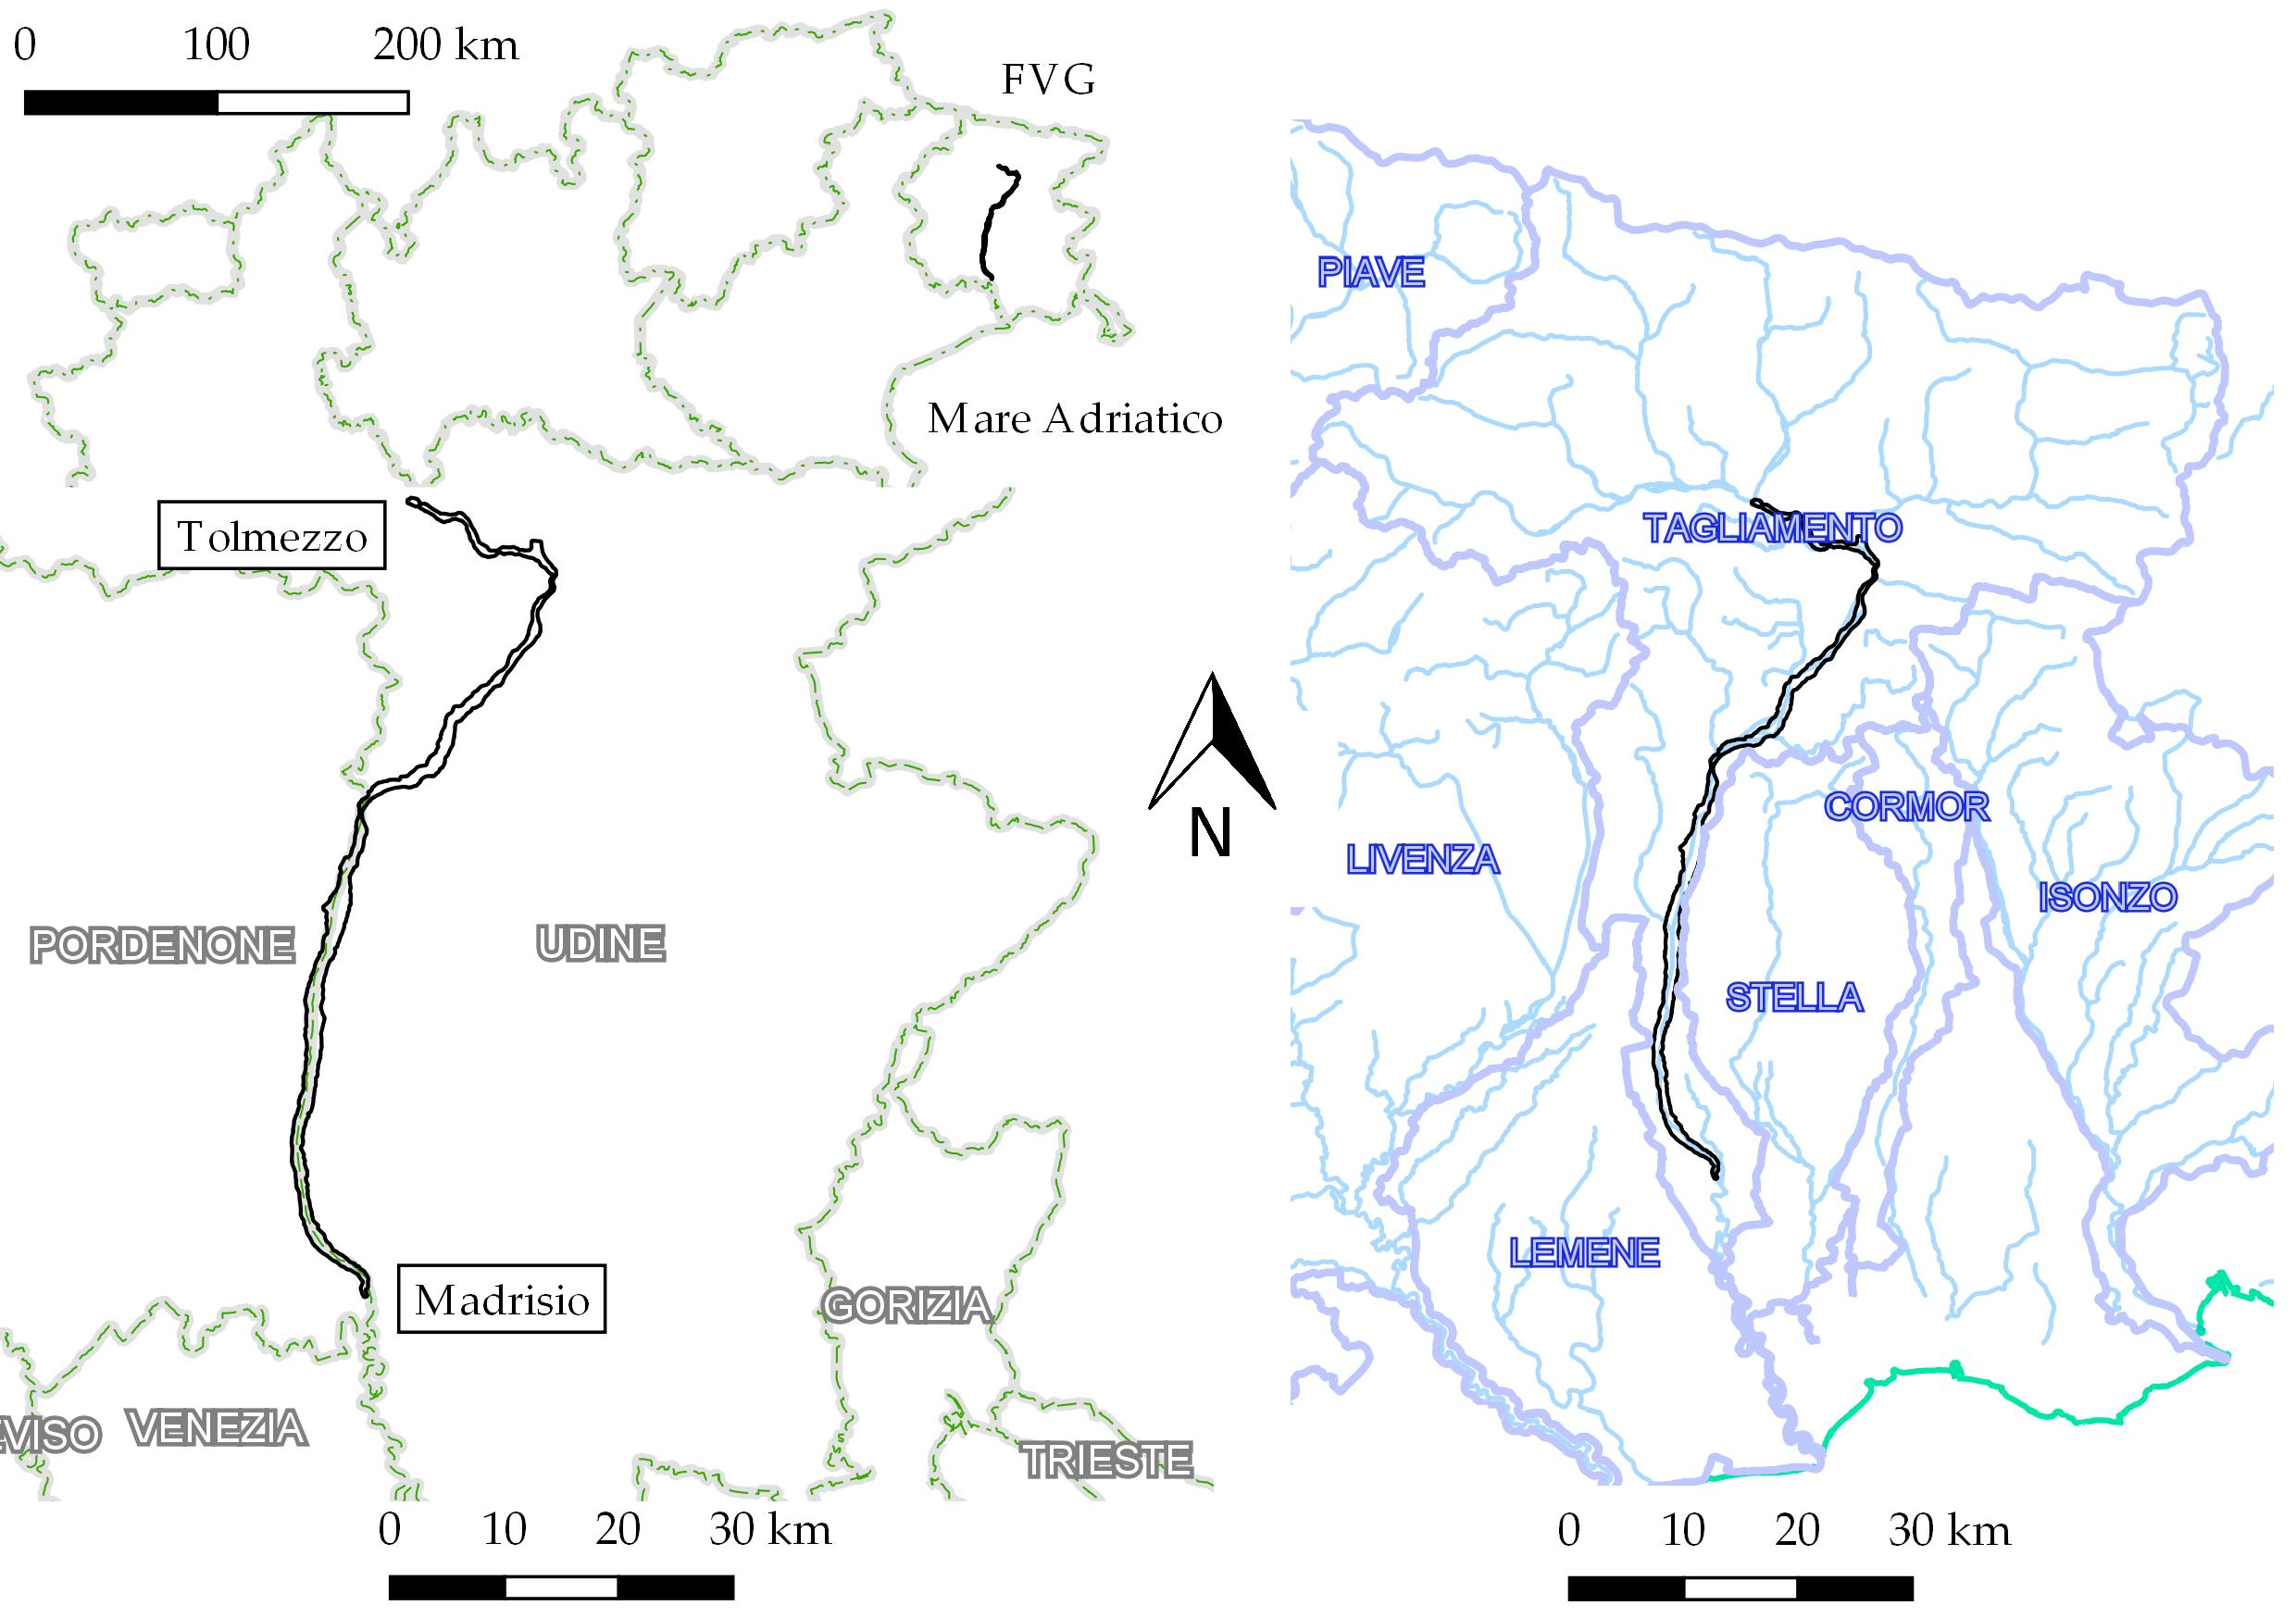
\includegraphics[width=\textwidth]{files/overview.jpeg}
	\caption[inquadramento dell'area di studio]
		{inquadramento dell'area di studio (poligono nero); a sinistra è mostrata l'Italia settentrionale (in alto) e un ingrandimento delle province e degli estremi dell'area di studio (in basso); a destra si vede il bacino idrografico del Tagliamento e di altri fiumi nelle vicinanze (in blu), il reticolo idrografico (in azzurro) e la linea di costa (in verde acqua).}
	\label{fig:overview}
\end{figure}
%
\begin{figure}
	\centering
	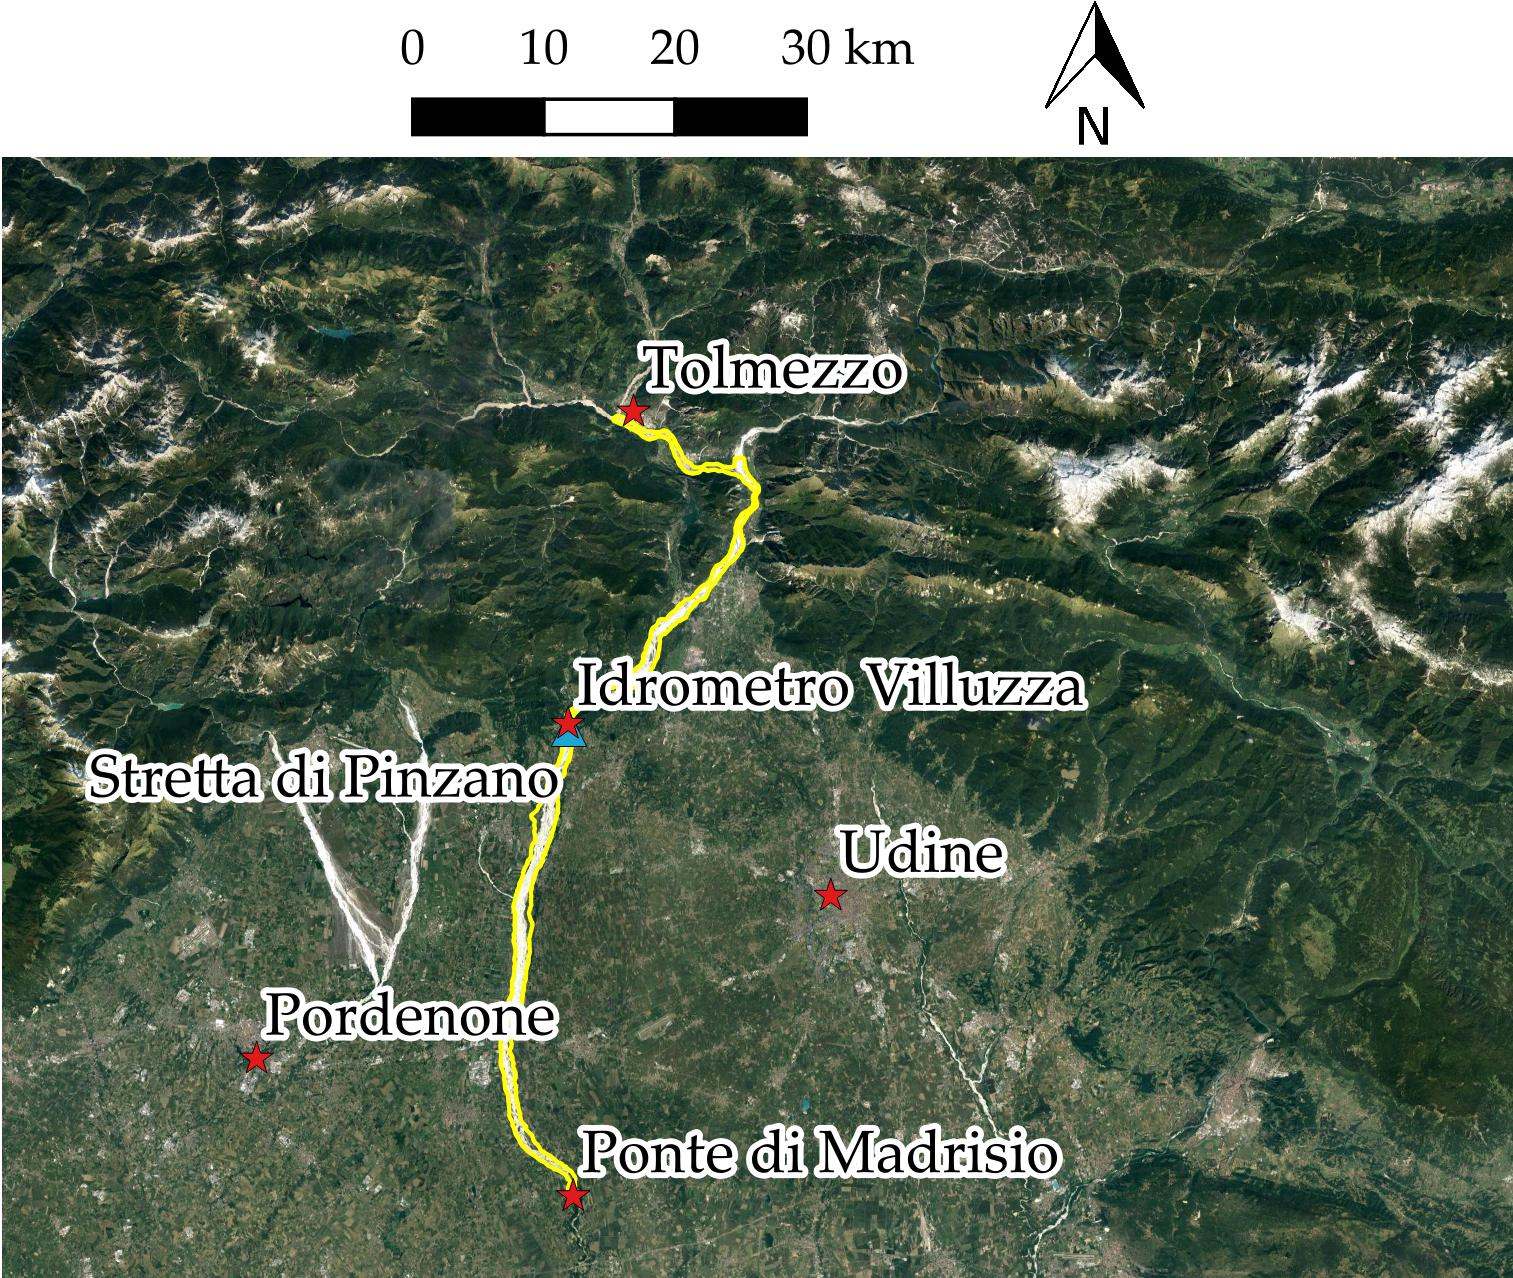
\includegraphics[width=\textwidth]{files/overview_tratto_sat.jpeg}
	\caption[inquadramento dell'area di studio]{inquadramento dell'area di studio (contornata in giallo).
	\\
	Map data: Google, Digital Globe.}
	\label{fig:overview-sat}
\end{figure}
%
\\
L'area di studio è stata suddivisa manualmente in 23~tratti con 22~sezioni al fine di avere un maggior dettaglio spaziale delle dinamiche di vegetazione (\vref{fig:23-tratti}). 
Questi tratti sono stati selezionati in modo da possedere caratteristiche omogenee per portata e crescita della vegetazione; 
pertanto confluenze di immissari, bruschi restringimenti o allargamenti, inizio di pronunciato \emph{upwelling} o \emph{downwelling} ed evidenti cambiamenti di morfologia fluviale sono stati gli elementi per individuare le 22~sezioni che determinano i 23~tratti.
%
\begin{figure}
	\centering
	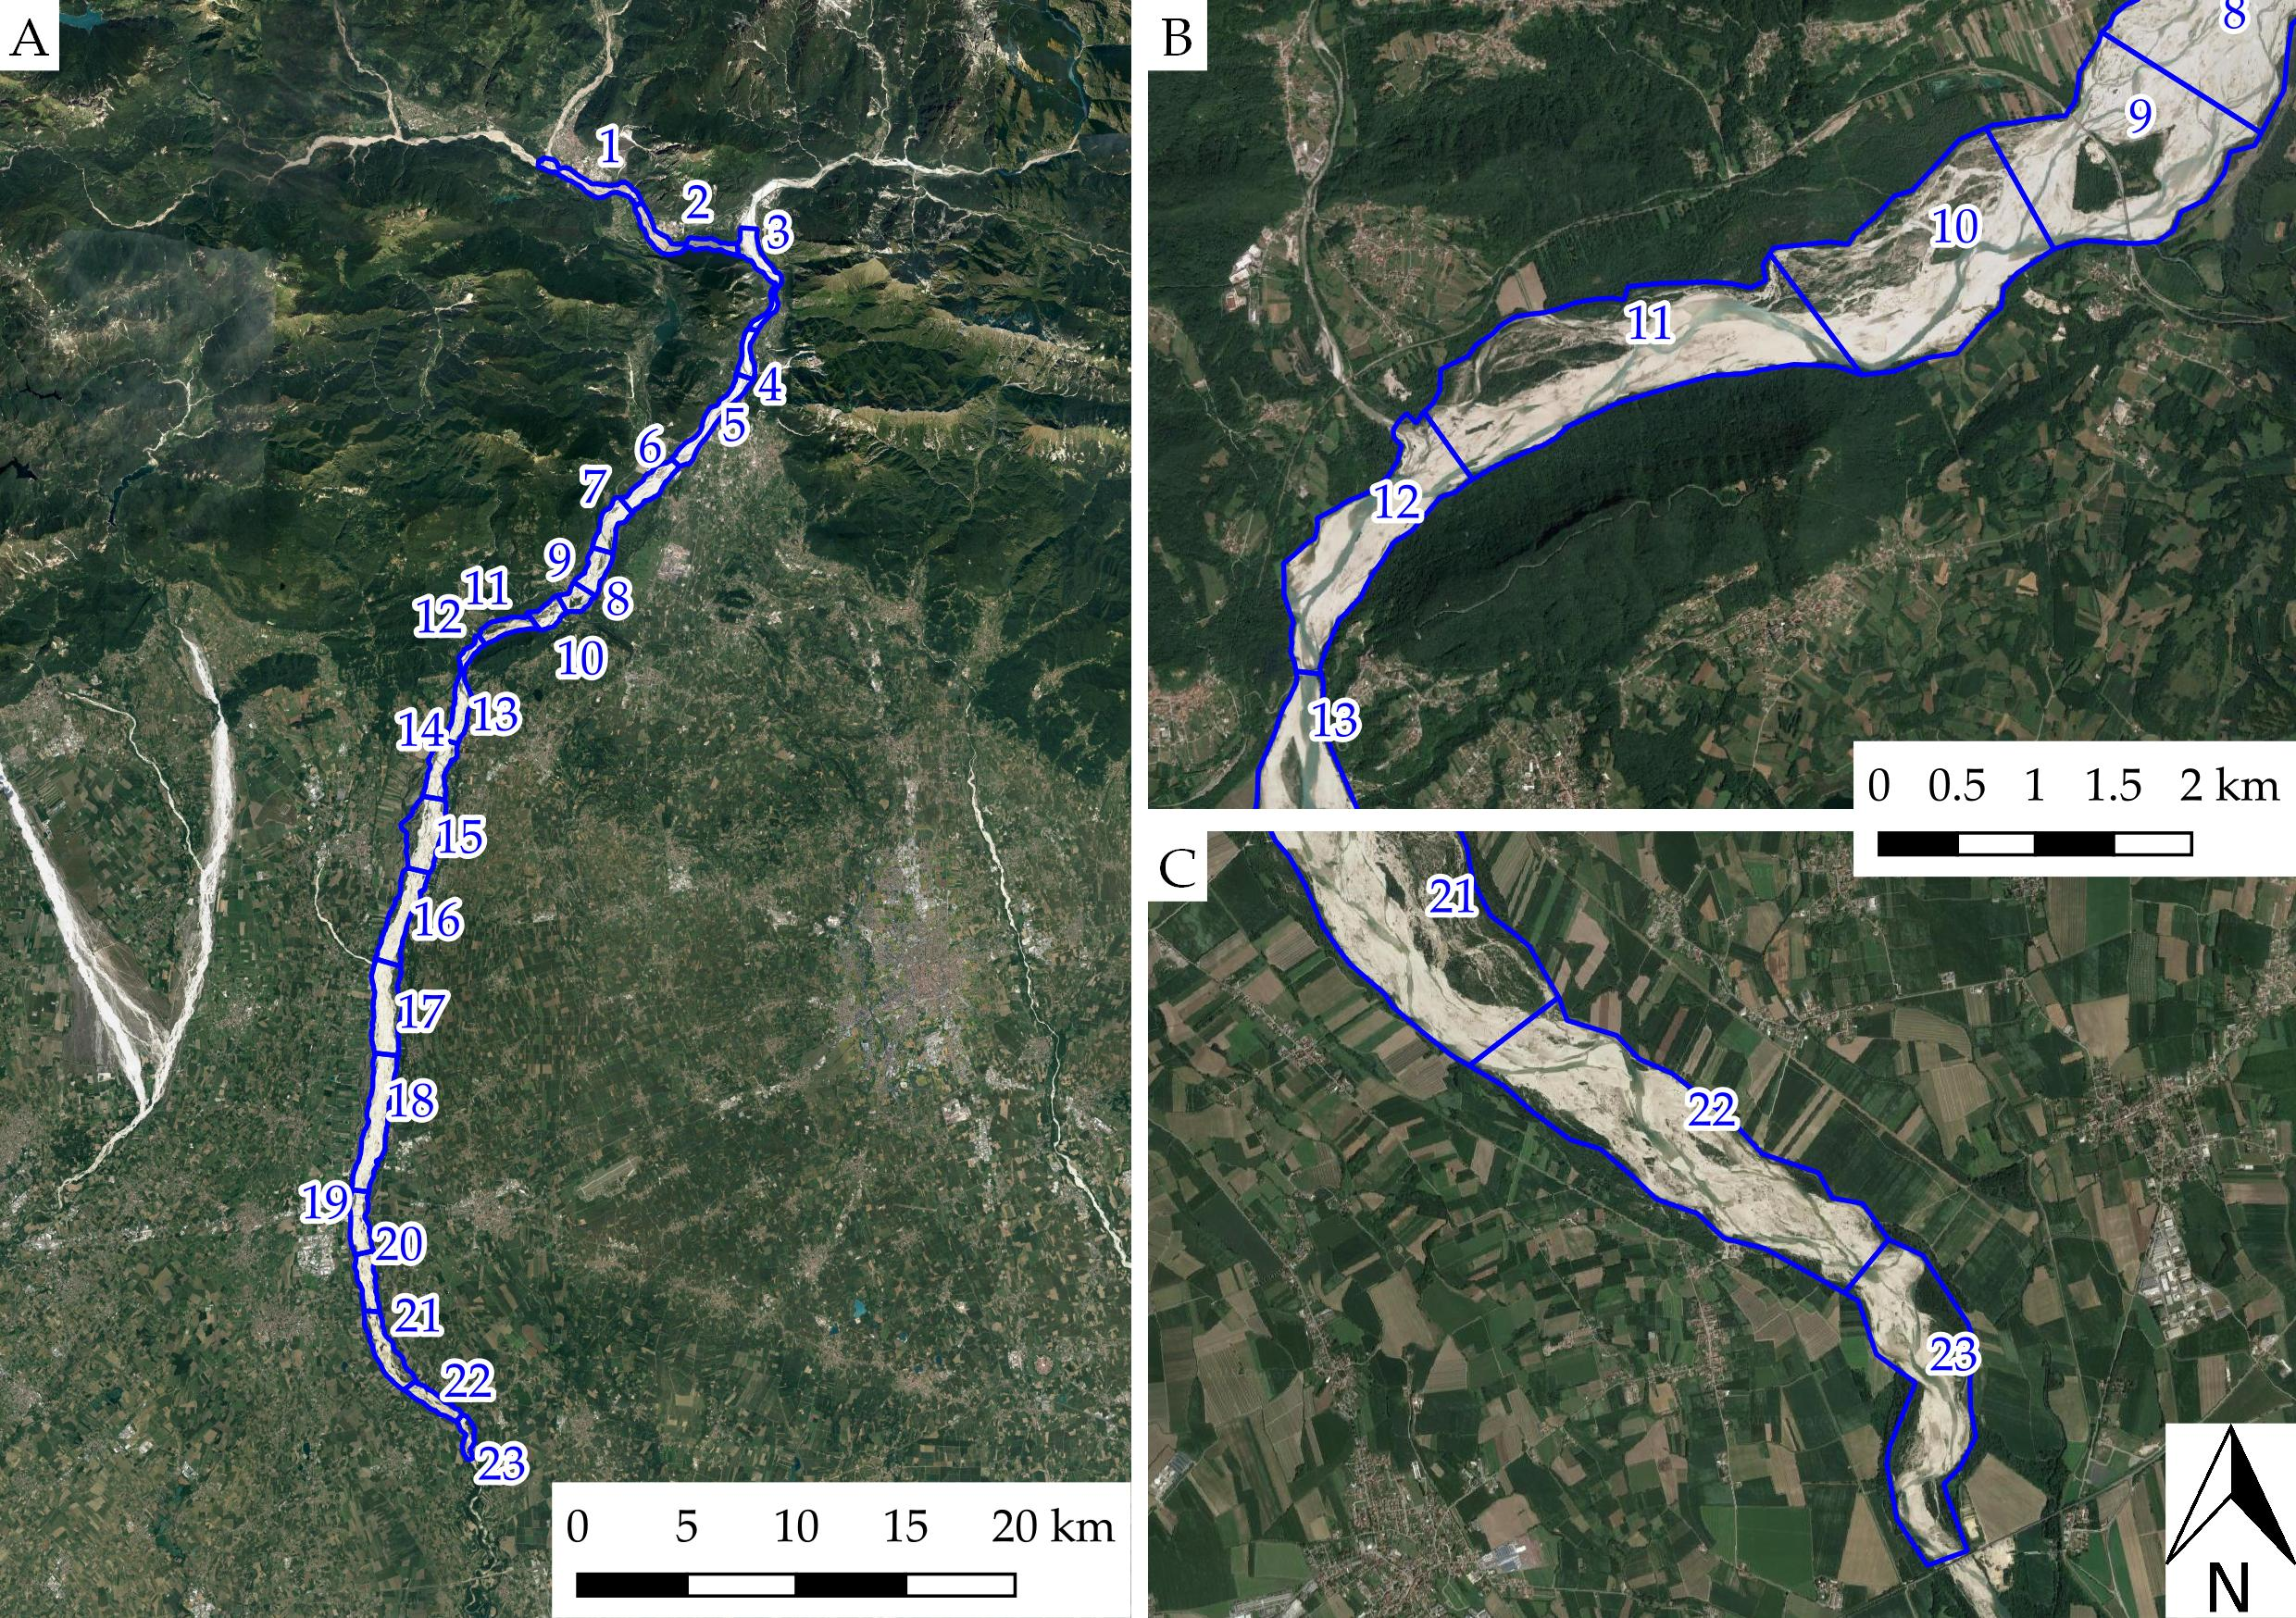
\includegraphics[width=\textwidth]{files/tutti_23_tratti.jpeg}
	\caption[i 23 tratti in cui è suddivisa l'area di studio]{i 23 tratti in cui è suddivisa l'area di studio (figura~A); la sezione di monte del tratto~1 corrisponde a Tolmezzo, la sezione di valle del tratto~23 corrisponde al ponte di Madrisio. A destra sono mostrati ingrandimenti dei tratti presso l'isola di Cornino e la stretta di Pinzano (figura~B) e nei tratti dove la morfologia diventa transizionale presso Madrisio (figura~C).
	\\
	Map data: Google, Digital Globe.}
	\label{fig:23-tratti}
\end{figure}


\section{Descrizione dell'area di studio}
\label{sec:descr-area-studio}

\paragraph{Connessione con la falda}
Nel tratto di studio nei pressi del paese di Pinzano al Tagliamento~(PN) è presente una stretta causata dall'affioramento di strati rocciosi che riduce la larghezza da diverse centinaia di metri a circa \SI{130}{\m}.
Questo restringimento, congiuntamente all'innalzamento dello strato di roccia che si trova sotto il letto del fiume, induce variazioni longitudinali nel livello di falda nel materasso alluvionale.
L'acqua filtrante da monte risale in alveo sottoforma di sorgenti diffuse: si assiste al fenomeno dell'\emph{upwelling}.
A valle della stretta, dove l'alveo non è più confinato e il letto roccioso sprofonda nel sottosuolo, l'acqua torna ad infiltrarsi nel materasso ghiaioso (\emph{downwelling}) tanto da portare il fiume in condizioni di secca in certi tratti quando non ci sono piene.
\\
L'\emph{upwelling} e il \emph{downwelling} sono fenomeni rilevanti durante i periodi di magra: certi tratti a valle della stretta di Pinzano possono essere in condizioni di secca, privi completamente di acqua, la quale scorre tutta nel sottosuolo e riemerge presso la “Linea delle risorgive”, quando la morfologia fluviale diventa transizionale vicino al ponte di Madrisio.
\\
Durante le piene questi fenomeni sono invece irrilevanti: l'acqua che emerge o che si infiltra contribuisce minimamente alla portata fluente.
\\
Inoltre il moto di infiltrazione contribuisce al mantenimento di una forte biodiversità caratteristica dell'ambiente fluviale, oltre a permettere una costante purificazione dell'acqua fluente in periodi di magra.

\paragraph{Affluenti}
Nel tratto di studio vi sono diversi affluenti (\vref{fig:affluenti}); vengono qui elencati da monte (Tolmezzo) fino a valle (Madrisio):
%
\begin{itemize}
	\item poco a valle di Tolmezzo c'è il Fella in sinistra idrografica (\SI{706}{\kilo\m\tothe{2}});
	\item all'altezza del paese di Venzone~(UD), in sinistra idrografica, sfocia il torrente Venzonassa (\SI{39}{\kilo\m\tothe{2}});
	\item qualche chilometro a monte del paese di Cornino~(UD) in destra idrografica c'è il Leale (\SI{100}{\kilo\m\tothe{2}}), le cui acque riempiono i canali incisi del Tagliamento che in magra sono quasi secchi;
	\item in corrispondenza dell'isola di Cornino in sinistra idrografica il Ledra (\SI{75}{\kilo\m\tothe{2}}) riporta nel corso del Tagliamento le acque che si sono infiltrate nella piana di Osoppo;
	\item immediatamente a monte della stretta di Pinzano in destra idrografica si getta l'Arzino (\SI{123}{\kilo\m\tothe{2}});
	\item infine, una decina di chilometri più a valle della stretta in destra idrografica si incontra il Cosa (\SI{160}{\kilo\m\tothe{2}}).
\end{itemize}
%
\begin{figure}
	\centering
	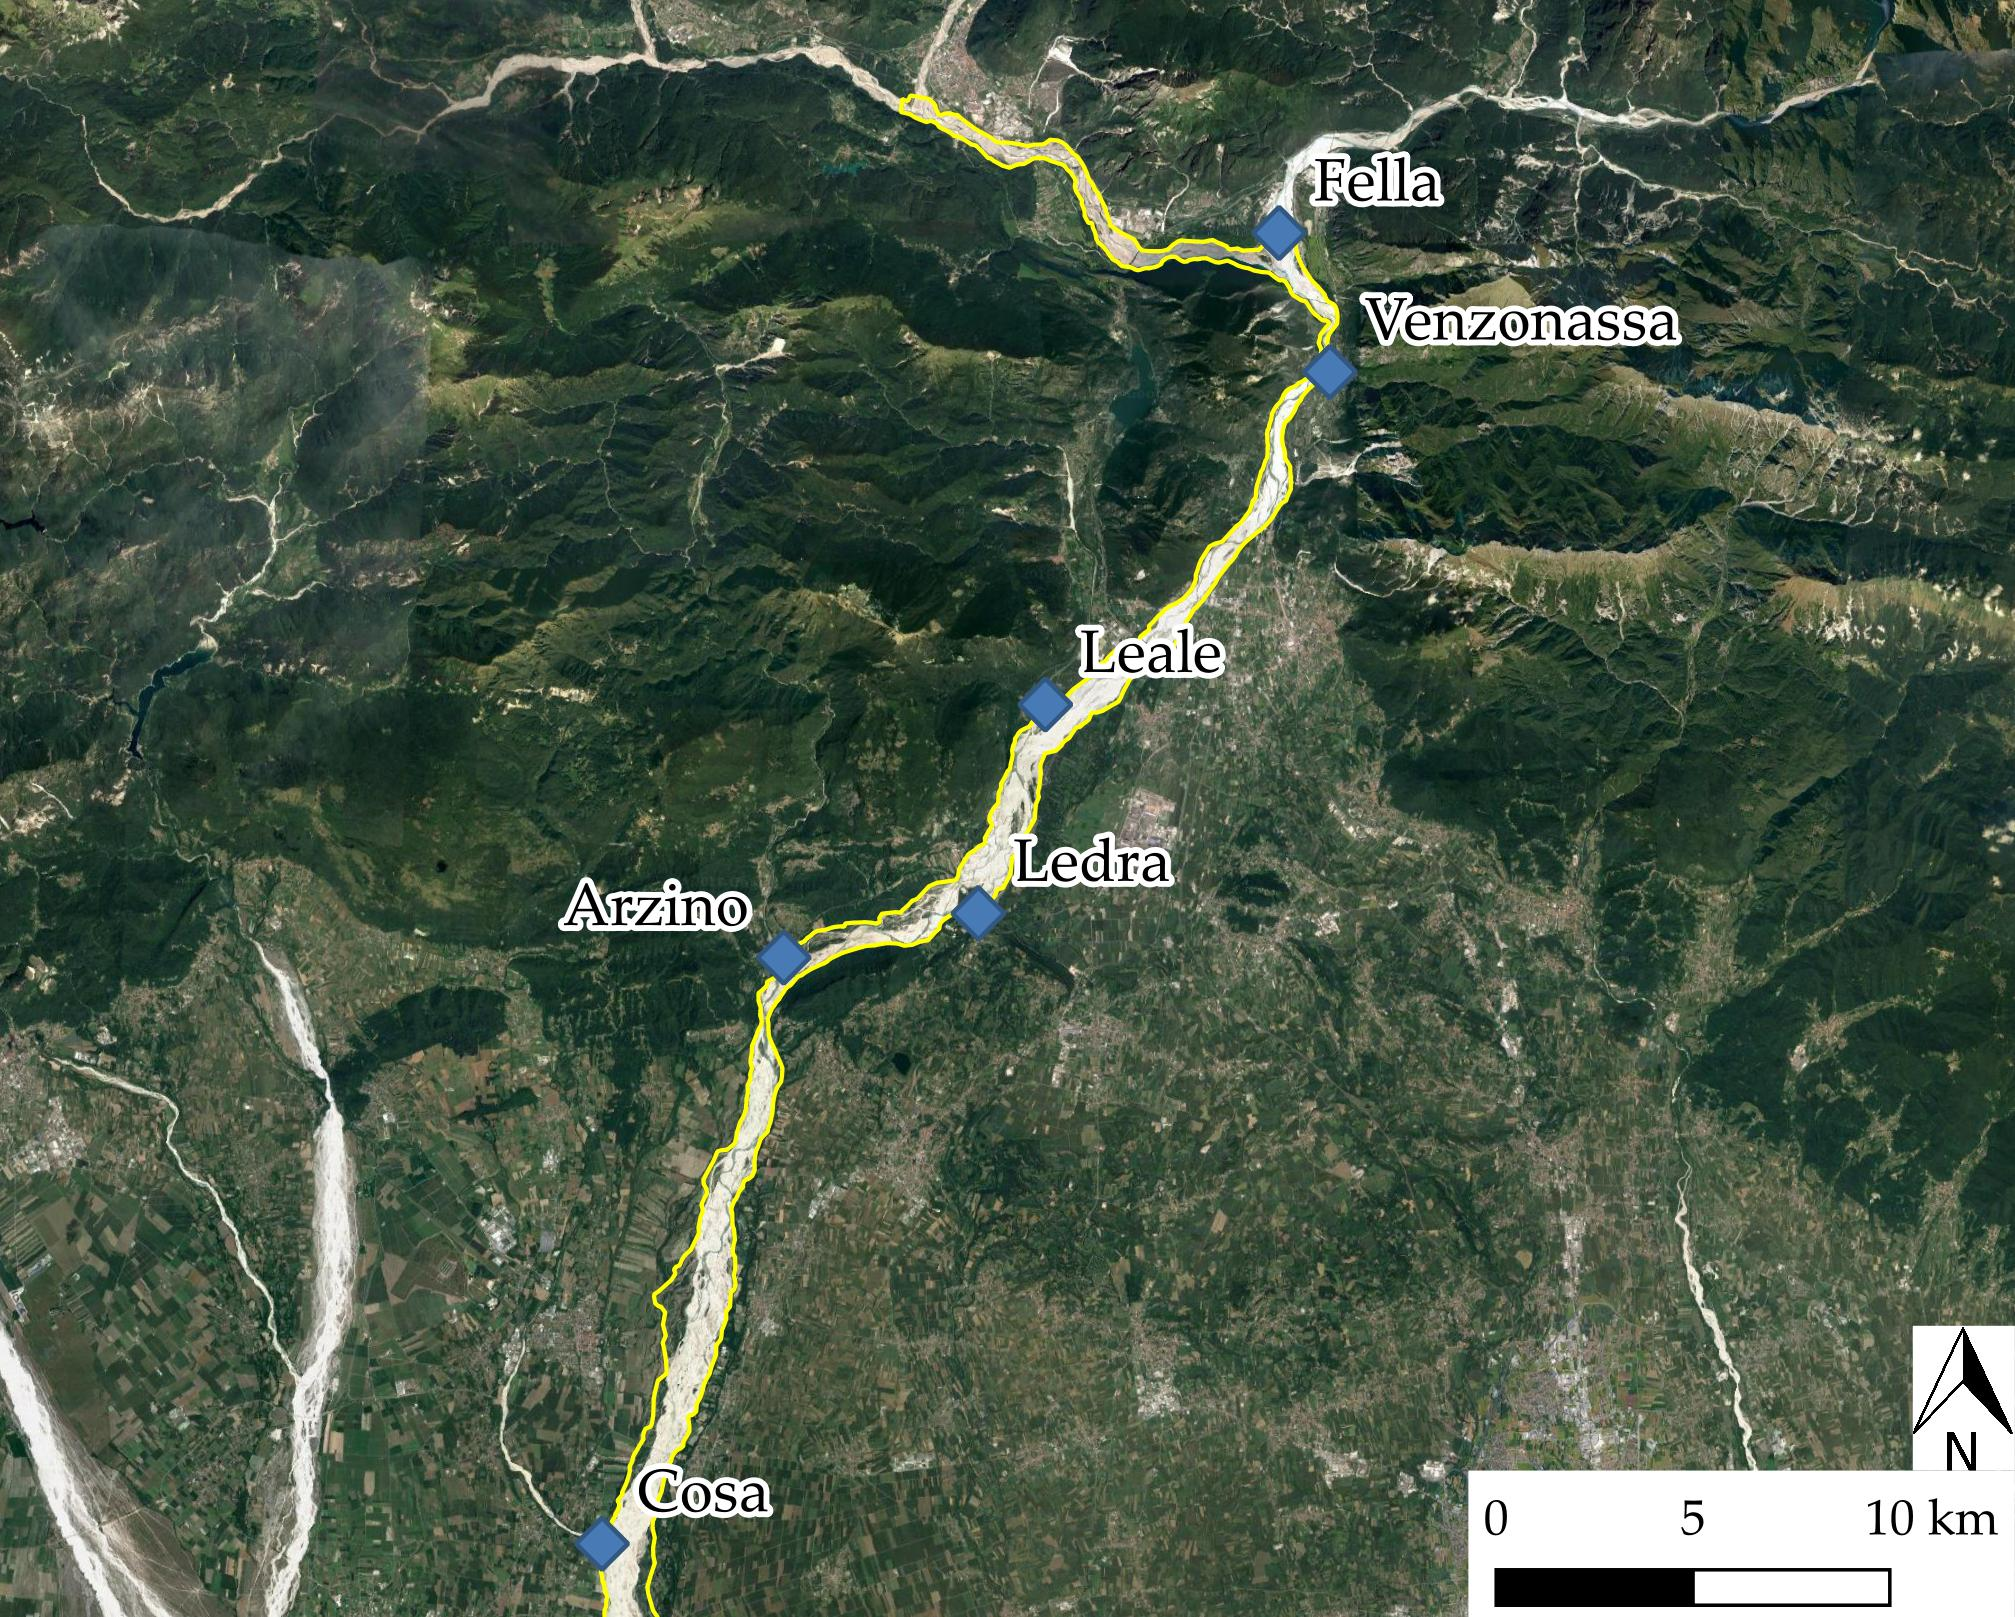
\includegraphics[width=\textwidth]{files/overview_affluenti.jpeg}
	\caption[principali affluenti nel tratto oggetto di studio]{principali affluenti nel tratto oggetto di studio (contornato in giallo).
	\\
	Map data: Google, Digital Globe.}
	\label{fig:affluenti}
\end{figure}
%
Il contributo di questi affluenti in termini di portata non è trascurabile; tuttavia è raro che eventi di piena abbiano luogo contemporaneamente in tutti i sottobacini tanto da incrementare sensibilmente il livello d'acqua nel Tagliamento a valle degli affluenti durante una piena.
Si ritiene pertanto che conoscere il livello d'acqua in un punto del Tagliamento sia sufficientemente rappresentativo per descrivere l'entità di una piena in tutto il tratto di studio; inoltre si assume che la portata fluente sia proporzionale all'area drenante in ogni sezione del fiume.

\paragraph{Dinamiche vegetazionali}
Nel fiume sono presenti numerose isole, composte prevalentemente da ontani bianchi \emph{Alnus incana} nei tratti montani (oltre l'area di studio), pioppi \emph{Populus nigra} e numerose specie di salice\emph{Salix spp.} nei tratti intermedi e vallivi.
Un'isola è un'area discreta e ben definita dell'alveo ricoperta da vegetazione e circondata da ghiaia o da canali (\vref{fig:esempio-isola}) \squarecites{Gurnell:2001-island-formation}{Bertoldi:2009-2m}.
%
\begin{figure}
	\centering
	\begin{subfigure}[b]{0.37\textwidth}
		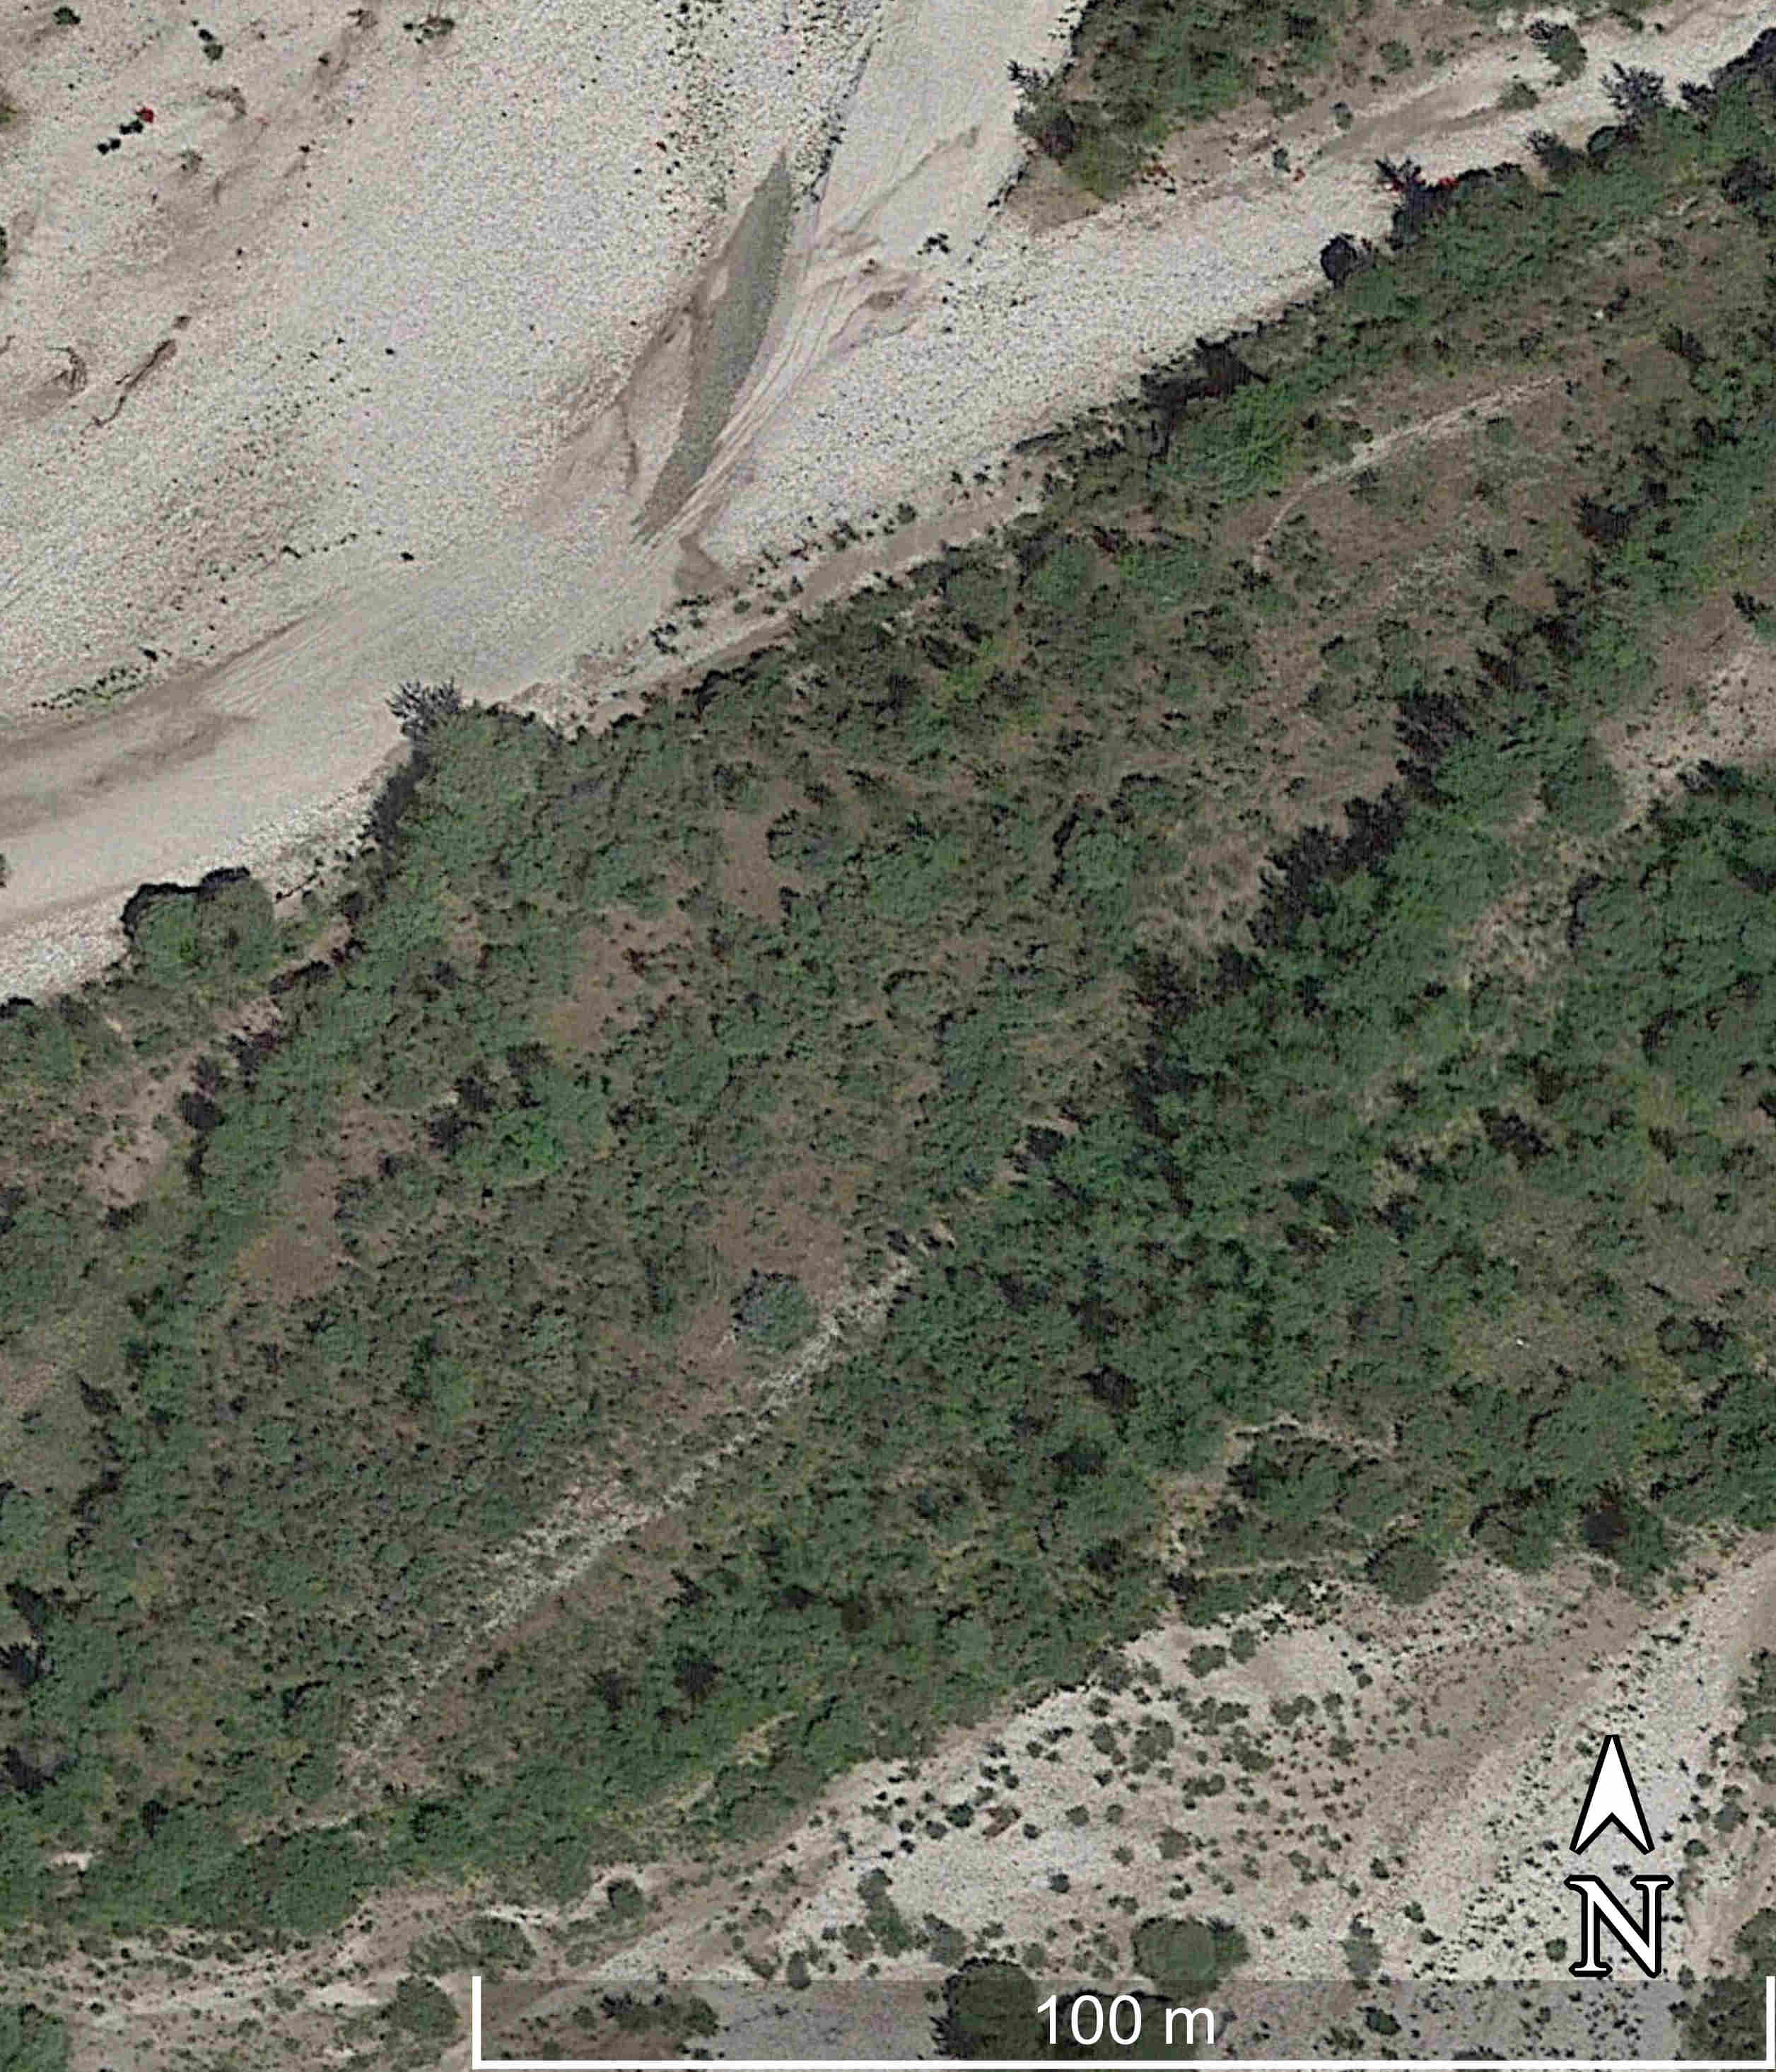
\includegraphics[width=\textwidth]{files/esempio_isola_sat_1.jpg}
		\caption{immagine da Google Earth di un isola in alveo.}
		\label{fig:esempio-isola-sat-1}
	\end{subfigure}
	\quad
	\begin{subfigure}[b]{0.57\textwidth}
		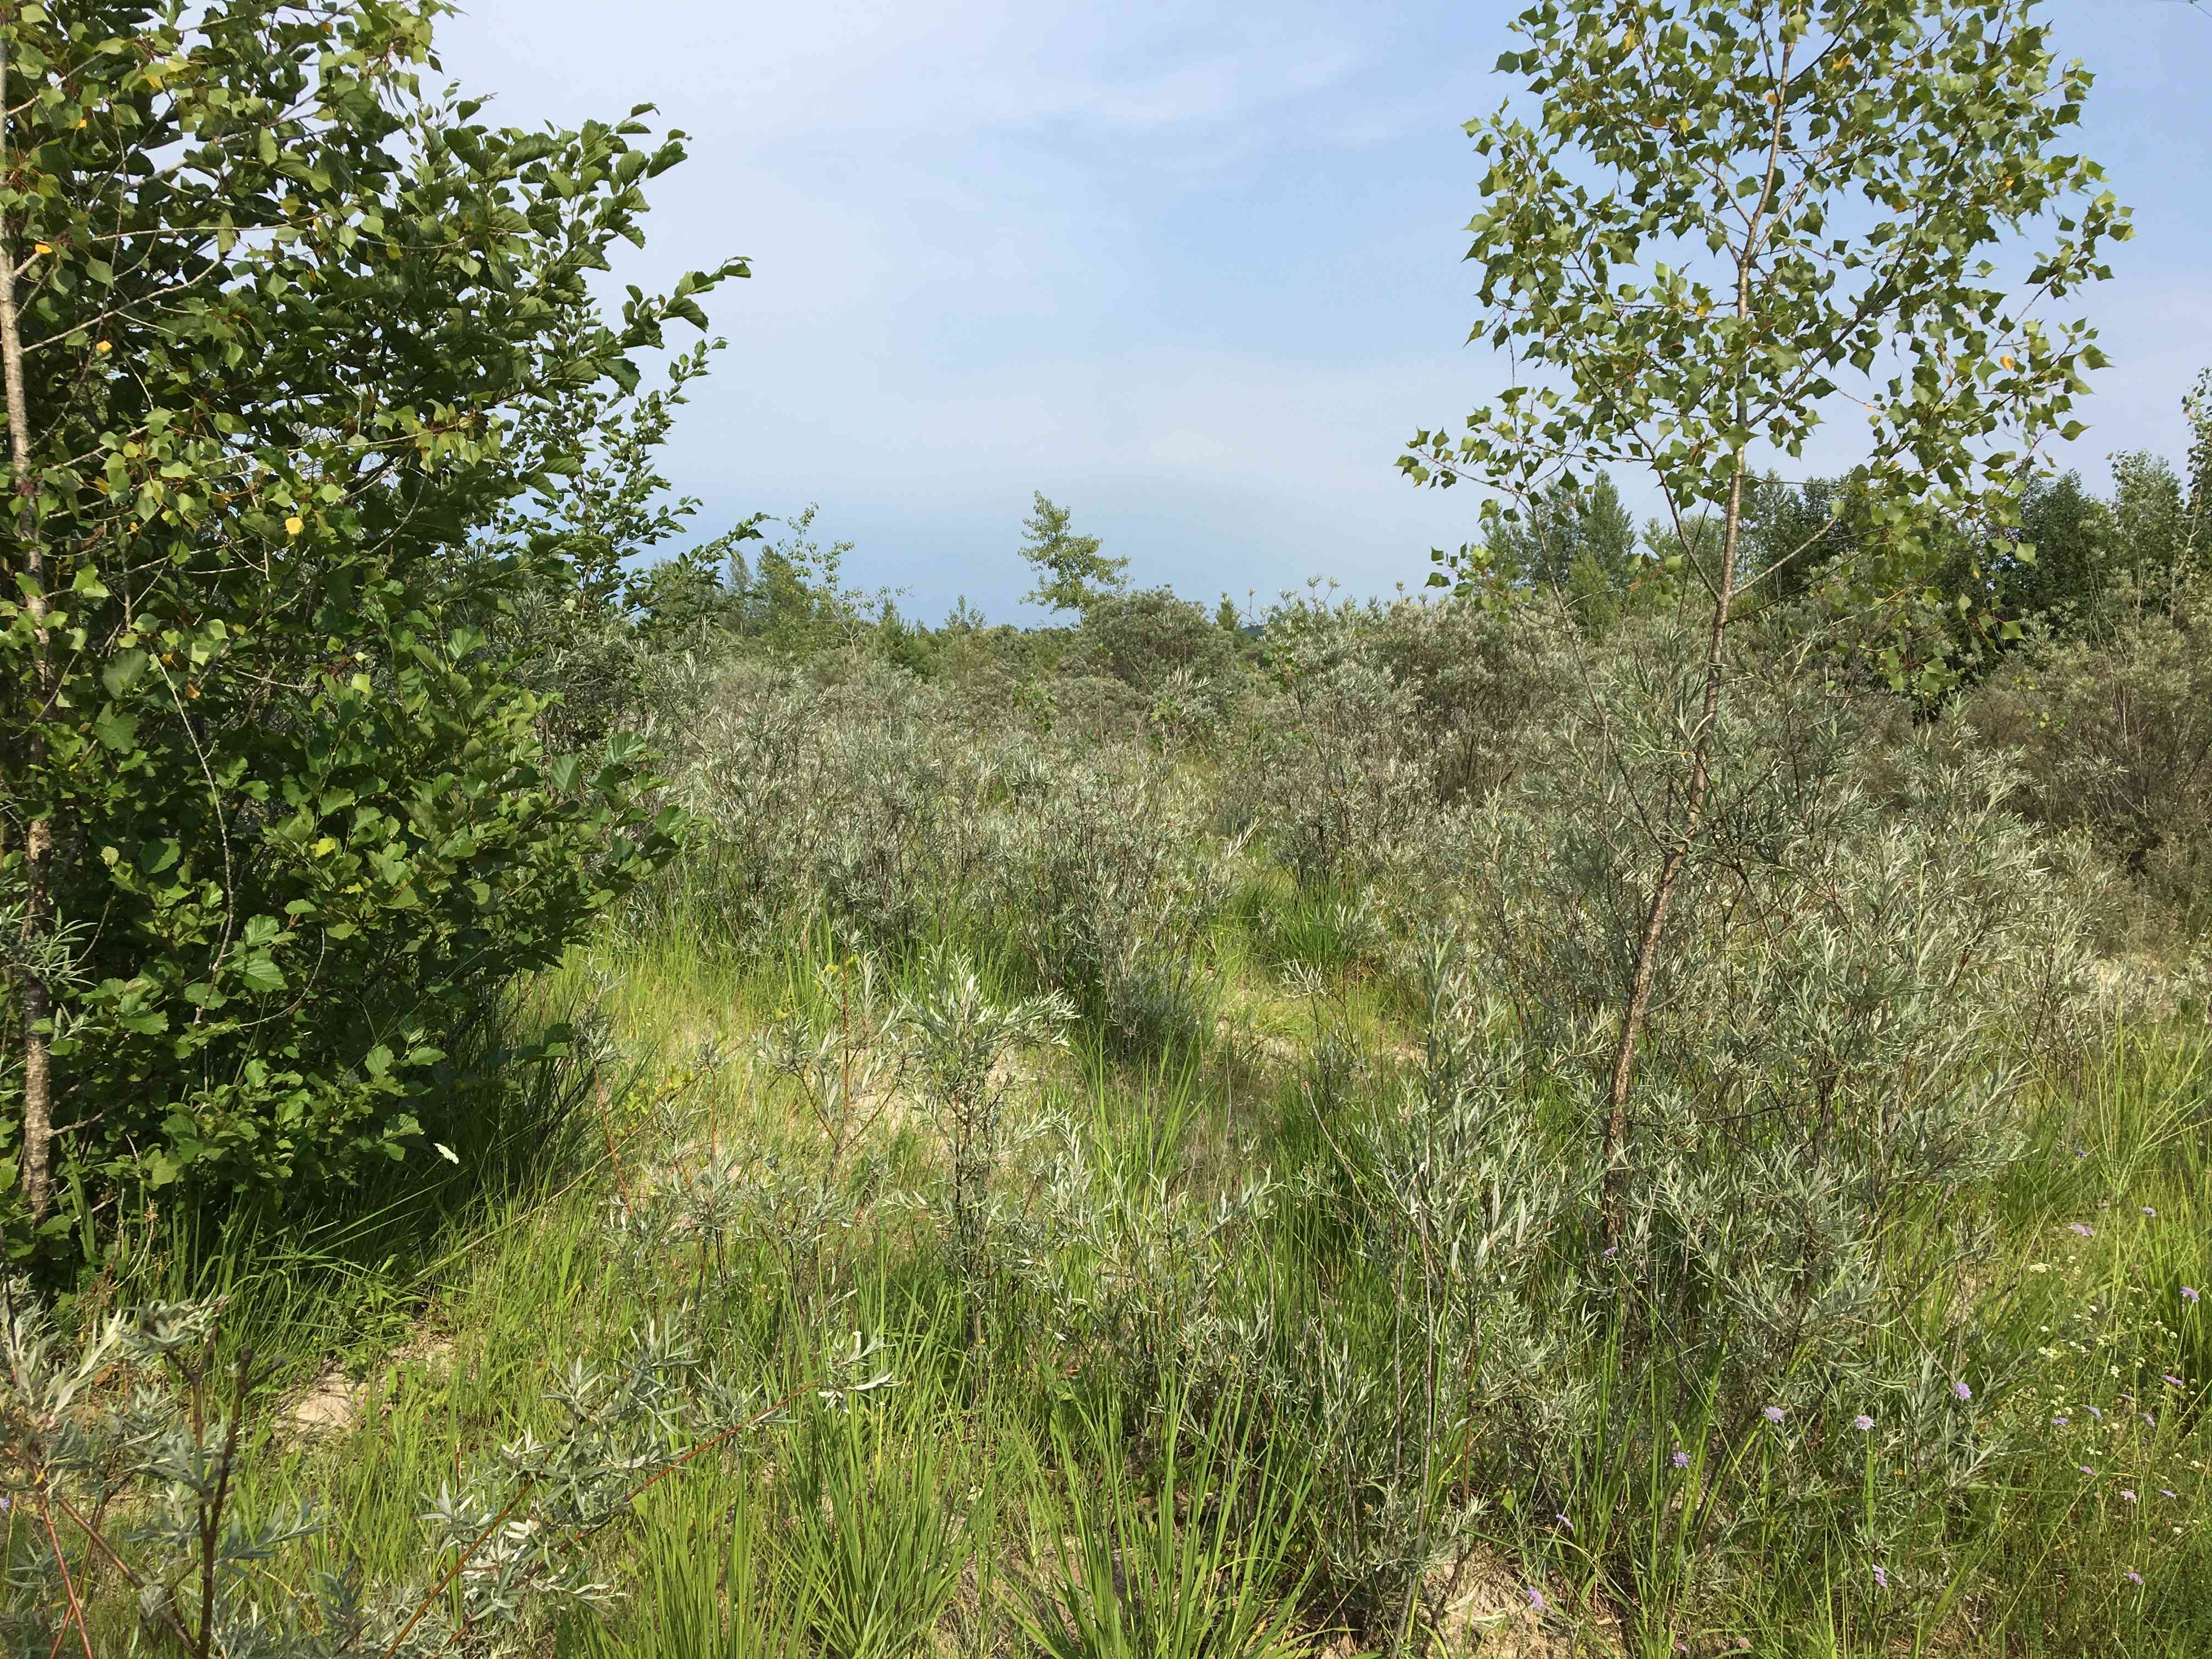
\includegraphics[width=\textwidth]{files/esempio_isola_1.jpg}
		\caption{foto di un isola molto vegetata presente nell'alveo del fiume.
		Foto dell'autore.}
		\label{fig:esempio-isola-1}
	\end{subfigure}
	\caption[immagine e foto di isole fluviali]{immagine e foto di isole fluviali; si noti la forte presenza di salici (\emph{Salix spp.}) e di pioppi (\emph{Populus nigra}); il luogo della foto è prossimo a quello dell'immagine.}
	\label{fig:esempio-isola}
\end{figure}
%
\\
Il meccanismo fondamentale di generazione di forme vegetate in alveo è la ricrescita vegetativa che caratterizza \emph{P. nigra} e \emph{Salix spp.}: i tronchi erosi e trasportati dalle piene e in seguito depositati sulla nuda ghiaia rigettano rami e foglie;
se vi è la contemporaneità di adeguate condizioni ambientali (non eccessiva velocità di abbassamento della falda in un substrato di pezzatura adeguata) ed idrologiche (frequenti piene di piccola-media entità, chiamate\emph{flow pulses}) allora i tronchi vivi crescono, intrappolano sedimenti e creano un buon ambiente per la successiva colonizzazione da parte di nuove piante (isole pioniere);
le isole si aggradano e accrescono caratterizzandosi con piante di diversa età (\emph{building island} e isole complesse) \squarecite{Gurnell:2001-island-formation}.
A loro volta la presenza delle isole influenza la posizione, grandezza, forma dei canali e le dinamiche del fondo.
\\
Si parla quindi di successione biogeomorfica nel corridoio fluviale attivo: l'ambiente fisico influenza la crescita delle piante coevolute con l'ambiente fluviale; queste a loro volta influenzano l'ambiente fisico e la sua evoluzione, tanto da essere state chiamate “ingegneri ecosistemici” \squarecite{Gurnell:2014-plants-eng}.

Possono formarsi isole anche da piante nate da seme, anche se queste sono più esigenti in termini di condizioni ambientali ed idrologiche.
\\
Eventi a piene rive (\emph{bankfull}) o più intensi possono dividere parti di vegetazione riparia dalla piana alluvionale, dando origine ad isole composte da piante mature coetanee, strutturalmente ben diverse dalle isole disetanee formate a partire da frammenti vegetativi.

Le isole sono distribuite disomogeneamente da monte verso valle: si può osservare che nei tratti con \emph{upwelling} il loro numero e la velocità di espansione crescono grazie all'acqua che risale dalla falda, mentre nei tratti con \emph{downwelling} la loro presenza diminuisce;
inoltre, nelle zone più strette come nei tratti montani o presso la stretta di Pinzano l'intensità della corrente è tale da ridurre o inibire la crescita di vegetazione, come mostrato da un modello concettuale in letteratura \squarecite{Gurnell:2014-plants-eng}.
\\
Temporalmente, le uniche isole che non vengono erose sono quelle che si fondono nella piana alluvionale; anche isole insediatesi da anni in alveo, aggradatesi fino a porsi a quote simili a quelle della \emph{floodplain}, possono essere completamente spazzate durante eventi \emph{bankfull} o maggiori.
Il tempo medio di persistenza di un'isola è di \SIrange[range-phrase={-}]{15}{20}{\anni}.
%TODO cita questo fatto!.


\section{Stato dell'arte}
Articoli precedentemente pubblicati hanno studiato l'ecologia e la morfodinamica del Tagliamento, le interrelazioni tra piante e fiume, la crescita della vegetazione riparia, la localizzazione delle isole in questo contesto naturale e molto altro.
\\
Inerentemente alla presente tesi, si riportano alcuni lavori di carattere simile o con risultati rilevanti rispetto all'argomento trattato.

Alcuni articoli si sono basati su immagini aeree e indagini di campo \squarecites{Zanoni:2008}{Bertoldi:2010-d50}{Surian:2015}: da una parte questi permettono la raccolta di informazioni in grande dettaglio, ma con risoluzione spaziale modesta (i rilievi aerei hanno un costo non indifferente) e risoluzione temporale particolarmente limitata (da pochi anni a decenni tra ogni rilievo).
\\
L'utilizzo di immagini satellitari multitemporali a bassa e ad alta risoluzione su aree estese permette di avere una visione d'insieme dei fenomeni, così come di evidenziare differenze spaziali e temporali.
Infatti è già stato dimostrato che è possibile estrarre risultati significativi sulla vegetazione riparia e sulle sue dinamiche da immagini satellitari a bassa risoluzione \squarecites{Bertoldi:2011-ASTER}{Henshaw:2013-LandSat}.
Questi lavori tuttavia hanno utilizzato delle maschere fisse per delimitare l'area attiva, senza distinguere in ogni immagine le isole dalla \emph{floodplain}.
\\
Degli autori hanno inoltre formulato modelli concettuali sulle dinamiche vegetazionali nei fiumi, in particolare nel Tagliamento \squarecites{Gurnell:2001-island-formation}{Gurnell:2006-omega}{Gurnell:2014-plants-eng}.
\\
Generalmente, il tratto più frequentemente studiato è quello compreso tra il ponte autostradale di Braulins~(UD) e la stretta di Pinzano.

Alcuni lavori hanno presentato risultati che questa tesi amplia e corrobora: tracciamento della traiettoria evolutiva della larghezza del fiume nel corso degli ultimi decenni o degli ultimi due secoli, osservazione della proporzione tra isole e alveo attivo \squarecites{Zanoni:2008}{Bertoldi:2011-ASTER}{Surian:2015}, ricerca di una relazione tra isole erose e portata \squarecite{Surian:2015}.

Infine, rispetto all'oggetto di ricerche precedenti e alle metodologie adottate questa tesi mira a:
%
\begin{itemize}
	\item utilizzare immagini a risoluzione temporale relativamente elevata validando i risultati attraverso rilievi aerei, di campo e dati da letteratura;
	\item analizzare un tratto di fiume più esteso rispetto a lavori simili;
	\item formalizzare alcuni dei modelli concettuali precedentemente elaborati;	
	\item mostrare che è possibile effettuare un monitoraggio delle dinamiche fluviali quasi in tempo reale. 
\end{itemize}

\section{Convenzioni}
Le seguenti convenzioni saranno utilizzate nella presente tesi:
\begin{description}
	\item[Mappe] riportate secondo WGS84/UTM~33N (EPSG:~32633);
	\item[Direzione della corrente] riportata con una freccia blu nelle immagini;
	\item[Formato delle date] AAAA-MM-GG;
	\item[Citazioni] sono nel formato Autore/i-Anno, racchiuse tra parentesi quadre;
	\item[Web link] sono riportati in note a piè pagina;
	\item[Termini in lingua straniera] sono in corsivo;
	\item[Glossario] presente nel materiale finale.
	%
\end{description}

